\documentclass[main.tex]{subfiles}

%\externalcitedocument{bibfile}

\begin{document}


\section{Neutrinos: A Primer}
Neutrinos make up three of the seventeen known fundamental particles to exist in nature, shown in Figure~\ref{fig:party}
\begin{figure}
    \centering
    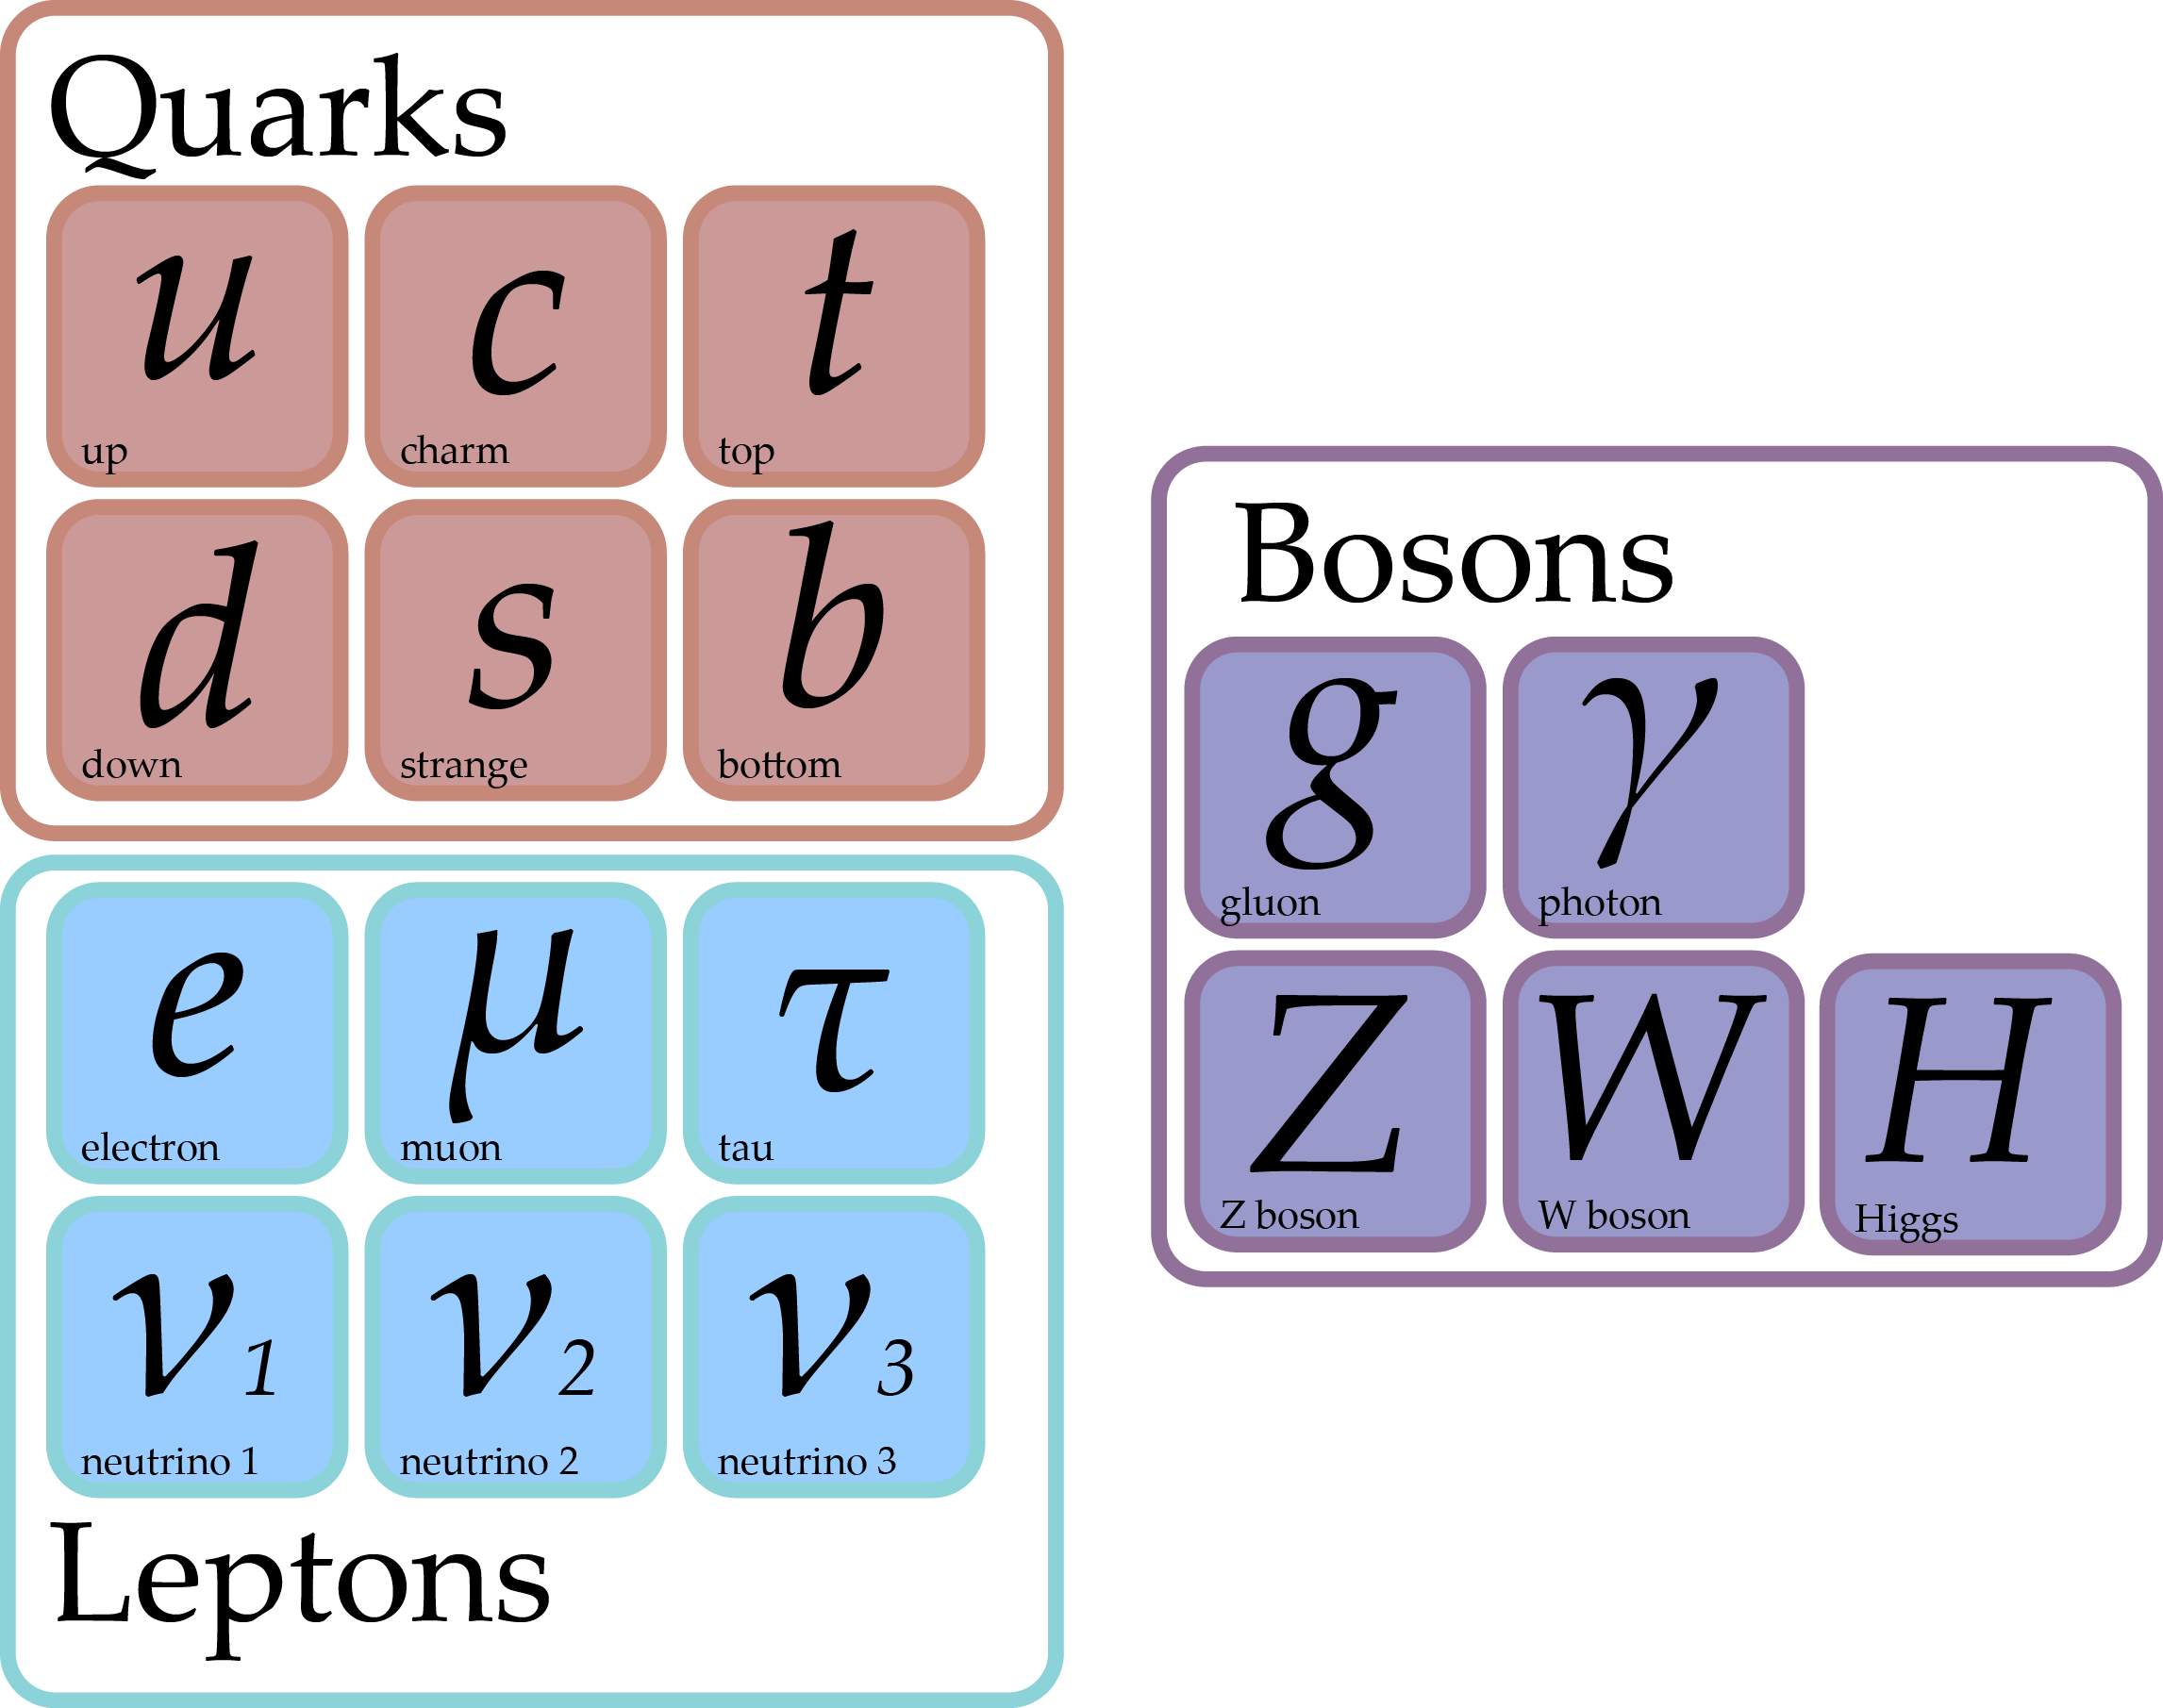
\includegraphics[width=0.8\linewidth]{figures/particles.png}
    \caption{A table of the seventeen fundamental particles. Only the mass-eigenstates for the fermions are shown.}\label{fig:party}
\end{figure}
The three-mass and three active-flavor neutrino \index{neutrino} paradigm has been well-studied~\cite{PhysRevD.98.030001,Esteban_2019,de_Salas_2018,Capozzi_2016,zboson2006, berns2021recent}, and is the conventional understanding.
At least two are known to be massive, but as of the time of writing there exist only upper bounds on their masses, and it is uncertain by which mechanism neutrinos get their mass.

However, several anomalies persist at short baselines, including in $\nu_\mu\rightarrow\nu_e $ appearance in decay-in-flight~\cite{aguilar2018significant} and decay-at-rest~\cite{Athanassopoulos_1998} beams  and $\nu_e\rightarrow\nu_e$ disappearance at reactors~\cite{mention2011reactor,serebrov2019first}  and with $^{71}$Ga electron capture sources~\cite{PhysRevC.73.045805,giunti2011statistical}.  
These anomalies have been attributed to possible oscillations of unknown neutrinos with mass-squared differences in the range of $\Delta m^{2}\sim 0.1-10\text{ eV}^{2}$~\cite{abazajian2012light}.   
Such an additional neutrino flavor state must be non-weakly interacting, or ``sterile,'' to be consistent with observed decay widths of the Z-boson~\cite{zboson2006}; the simplest such model is known as the ``3+1'' light sterile neutrino model in which a single sterile neutrino is added. 

There have been interesting recent developments for the 3+1 model.  
The BEST experiment appears to validate the anomalous electron neutrino disappearance signature of the previous gallium anomalies with a new level of statistical significance and experimental precision~\cite{barinov2021results}. 
The Neutrino-4 experiment claims evidence of short-baseline oscillations in the $\bar{\nu}_e$ disappearance channel with $\Delta m^2\sim 7.3\,\mathrm{eV}^2$ at the 2.9$\sigma$ level.
 Meanwhile results from the MicroBooNE~\cite{microboonecollaboration2021search,microboonecollaboration2021search1,microboonecollaboration2021searchmulti} experiment challenge the interpretation that the MiniBooNE low energy excess~\cite{miniboone2018} is due entirely to the electron neutrino by placing a constraint on the sterile neutrino interpretation of the excess; though the impact of this observation on the 3+1 model has yet to be assessed.  Continued exploration of sterile neutrino mixing in all channels and all energy ranges thus remains strongly motivated~\cite{sbnfermilab}.

The addition of a fourth neutrino mass and flavor eigenstate expands the unitary mixing matrix to four dimensions. 
The four-neutrino oscillations model becomes an extension of the three-neutrino model with three additional mixing angles $\theta_{14}$, $\theta_{24}$, and $\theta_{34}$, and two new CP-violating phases $\delta_{14}$ and $\delta_{24}$. These three new mixing angles parametrize the amplitude of oscillations between the three active states and the one sterile state, and lead to additional short-baseline vacuum-like oscillations as well as novel effects in the presence of matter~\cite{Akhmedov:1988kd,KRASTEV1989341,Chizhov:1998ug, Chizhov_1999, Akhmedov_2000, Nunokawa:2003ep,Petcov:2016iiu}.  In this work we consider CP-conserving models with all CP-violating phases set to zero.

Of particular interest to neutrino telescopes, matter effects can result in the near complete disappearance of TeV-scale muon anti-neutrinos passing through the Earth's core for a sterile neutrino with eV-scale mass squared differences~\cite{Nunokawa:2003ep, Choubey:2007ji, Barger:2011rc, Esmaili:2012nz, esmaili2013restricting, Lindner:2015iaa}. This signature of matter-enhanced resonant disappearance has been targeted by the IceCube Neutrino Observatory~\cite{Aartsen_2020, Aartsen_2020_prd}, leading to one of the  most sensitive $\nu_\mu$ disappearance analyses to date. The result of the analysis was a closed 90\% contour with best fit point at $\sin^2 2\theta_{24}\sim0.1$ and $\Delta m^2_{14}=4.5\text{ eV}^2$, under a conservative assumption (for the $\nu_\mu$ disappearance channel) that $\theta_{34}=\theta_{14}=0$. In addition to being a strong refutation, lower mass solutions consistent with the LSND~\cite{Athanassopoulos_1998} and MiniBooNE anomalies and constraints around 1~eV$^2$~\cite{kopp2013sterile, Cirelli:2004cz, abazajian2012light, Gariazzo:2017fdh, Dentler:2017tkw, Diaz:2019fwt}, a possible interpretation of this result is as a statistically weak hint of a disappearance signature around $\Delta m^2_{41}\sim4.5\text{ eV}^2$.  Further exploration of this region of parameter space  in other channels at neutrino telescopes is therefore strongly motivated. 

\subsection{Neutrino oscillations}
\index{neutrino!oscillations}

First, a review of how these oscillations happen is of merit. From the solar neurino problem CITE it is understood that neutrinos oscillate, and from that we understand they have mass. To understand \textit{why} that is the case we consider that the neutrinos mass and flavor eigenstates are not identical. That there is some unitary matrix, 
\begin{equation}
    U_{\text{PMNS}} = \left(\begin{array}{ccc} U_{e1} & U_{e2} & U_{e3} \\ U_{\mu 1} & U_{\mu 2} & U_{\mu 3} \\ U_{\tau 1} & U_{\tau 2} & U_{\tau 3} \end{array}\right)
\end{equation}
which allows for transformations from the mass basis to the flavor basis, such that
\begin{equation}
    \left(\begin{array}{ccc} \nu_{e} & \nu_{\mu} & \nu_{\tau} \end{array}\right)  = \left(\begin{array}{ccc} U_{e1} & U_{e2} & U_{e3} \\ U_{\mu 1} & U_{\mu 2} & U_{\mu 3} \\ U_{\tau 1} & U_{\tau 2} & U_{\tau 3} \end{array}\right) \left(\begin{array}{c} \nu_{1} \\ \nu_{2} \\ \nu_{3} \end{array}\right).
\end{equation}
where $\nu_{i}$, $i\in\left(1,2,3\right)$ is in the mass basis and $i\in\left(e,\mu\tau\right)$ is in the flavor basis. 
We can, in general then, express a stationary state in one basis in terms of the other basis:
\begin{equation}\label{eq:nunu}
    \ket{\nu_{e}} = U_{e1} \ket{\nu_{1}} + U_{e2} \ket{\nu_{2}} + U_{e3}\ket{\nu_{3}}.
\end{equation}
To consider a neutrino in-flight, we consider the time-dependent Schr\"odinger Equation
\begin{equation}
    i\dfrac{\partial}{\partial t} \ket{\nu_{i} (t)} = \bvec{H}_{\nu}\ket{\nu_{i}(t)},
\end{equation}
which can be solved with the stationary state solution 
\begin{equation}
    \ket{\nu_{i} (t)}  =  e^{-iEt} \ket{\nu_{i} (0)}.
\end{equation}
For neutrinos, we can expand out the energy term and simplify under the small-mass assumption. 
\begin{align}
    E_{i} &= \sqrt{p^{2}c^{2} + m_{i}^{2}c^{4}} \\
    &\approxeq pc + \dfrac{m_{i}^{2}c^{4}}{2E_{i}}
\end{align}
The stationary state solution then becomes 
\begin{equation}
    \ket{\nu_{i} (t)}  =  e^{-ipt}e^{ m_{i}^{2}/(2E}\ket{\nu_{i} (0)}
\end{equation}
and for the state described in Equation~\eqref{eq:nunu},

\begin{equation}
    \ket{\nu_{e}(t)} = \sum\limits_{i} U_{ei} e^{-ipt}e^{ m_{i}^{2}/(2E)}\ket{\nu_{i} (0)}
\end{equation}


Therefore, when considering a neutrino originally in the electron flavor state and at energy $E$, then propagated over a distance \(L\), we can calcualte the odds of measuring it in the same electron flavor state. This is the $P(\nu_{e}\to\nu_{e})$ survival probability. Expressed in the mass eigenstate, 


\subsection{3+1 Neutrino Oscillations}
\index{neutrino!oscillations}
An additional fourth neutrino mass an flavor eigenstate will modify exxpected oscillations. To parametrize this, three additional mixing angles and two additional CP-violating phases must be added to the standard three neutrino paradigm. The new four-neutrino unitary mixing matrix becomes.
\begin{equation}
    U_{\text{PMNS}} = \left(\begin{array}{cccc} 1 & 0 & 0 & 0 \\ 0&\cos\theta_{23}&\sin\theta_{23}&0 \\ 0&-\sin\theta_{23}&\cos\theta_{23}&0 \\ 0&0&0&1 \end{array}\right)
\end{equation}

\subsection{Neutrino Interactions}
\index{neutrino!interactions}
Discuss neutrino interactions at medium to high energies. Deep Inelastic Scattering

\subsection{Matter Effects on Neutrion Oscillations}
Words on the matter effect. \index{neutrino!matter effect} Effective neutrino masses. 




\end{document}